\section{Event Time-Series Creation}
\label{sec:4}
\begin{figure}[H]
\centering
    \label{fig:ts-creation}
    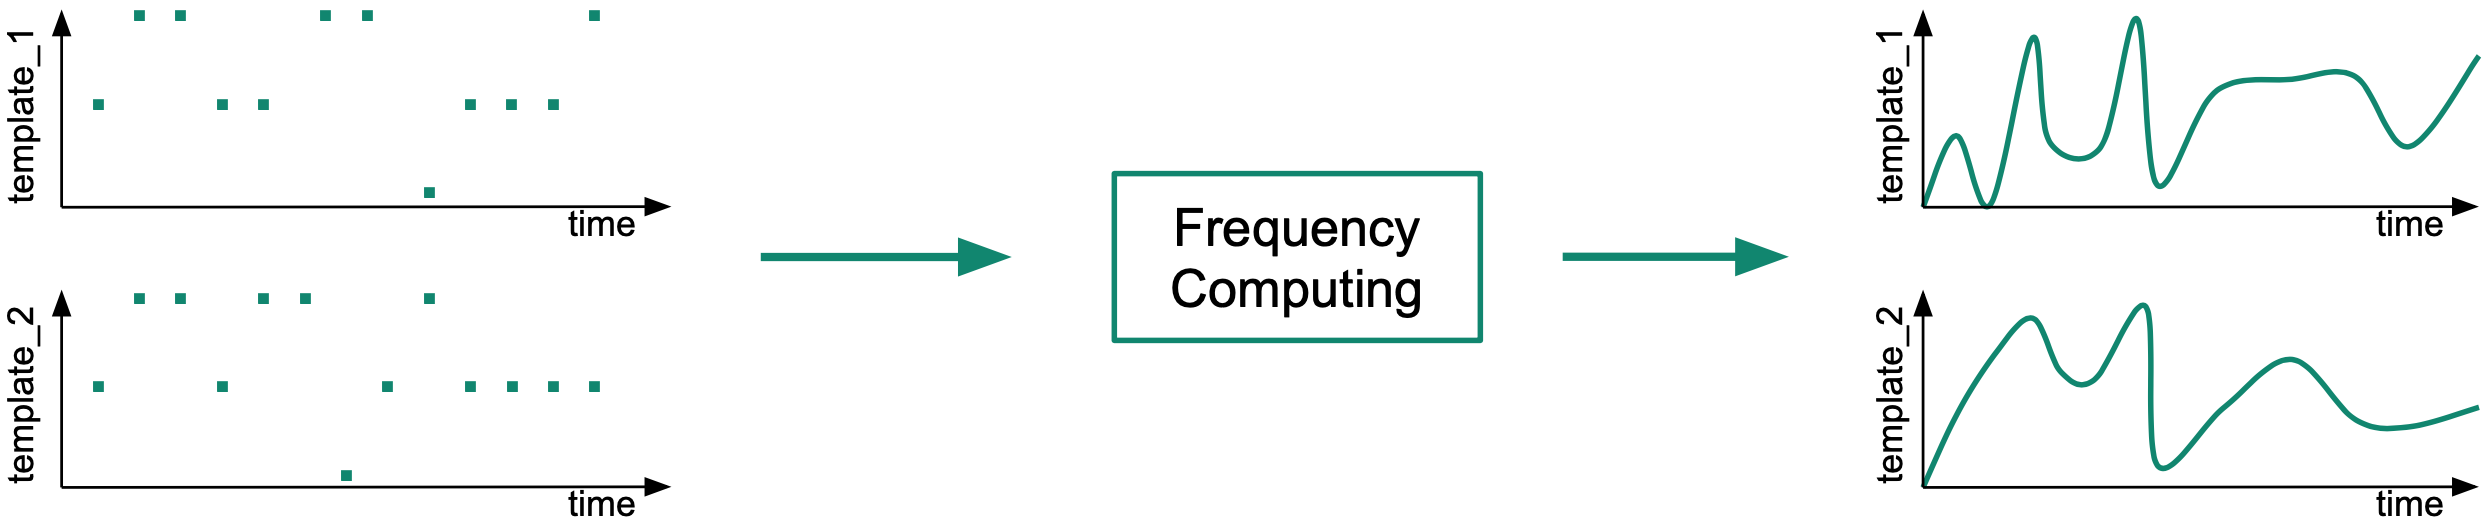
\includegraphics[width=\textwidth]{figures/ts_creation.png}
    \caption{The time-series creation flow.}
\end{figure}
After extracting the set of log templates, we construct a set of event time-series generated by each log template from all log data. In other words, we compute the frequency of log templates, that is, the number of appearances of one log template in each time bin (see also Figure \hyperref[fig:ts-strategies]{3}). This transformation from log space to metric space helps us run causal inference algorithms directly on information from log data \cite{jia2017approach}.
\begin{figure}[H]
\centering
    \label{fig:ts-strategies}
    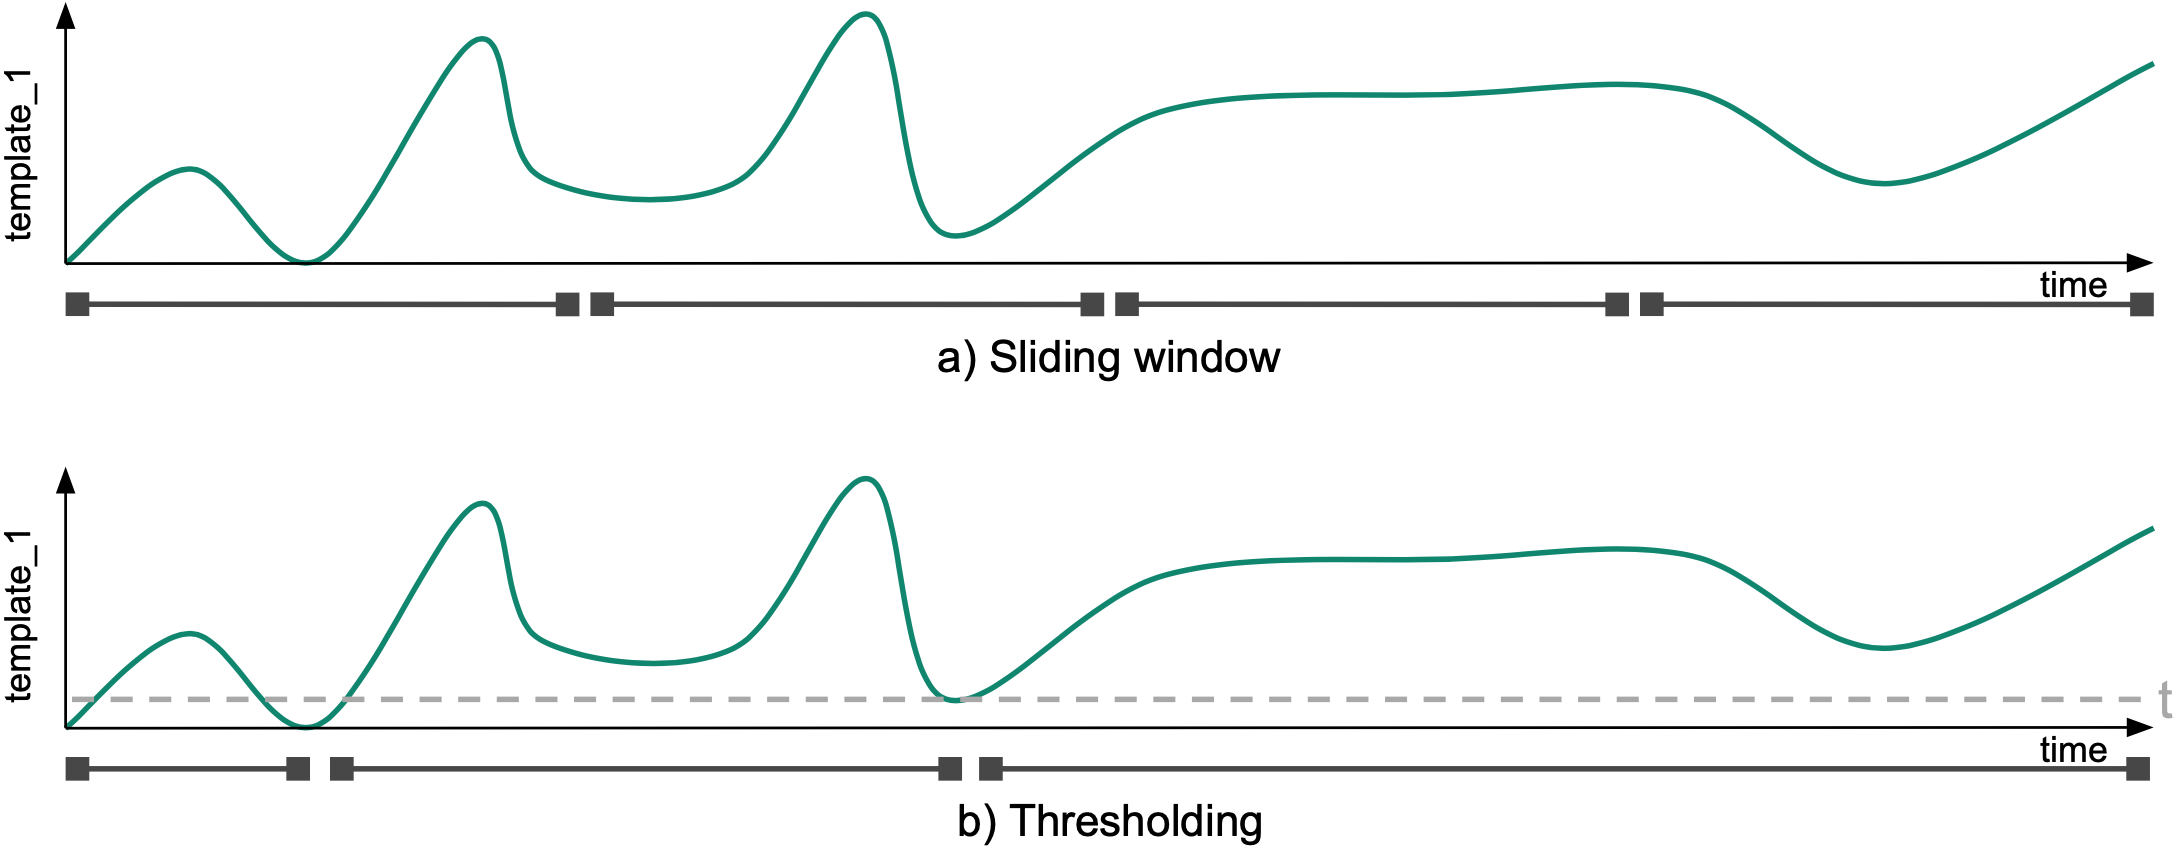
\includegraphics[width=\textwidth]{figures/ts_strategies.png}
    \caption{The time-series modeling strategies.}
\end{figure}
There are two main strategies for treating time-series data \cite{glymour2019review}. One is to partition the data into non-overlapping equals windows and take the measurements in each unit as an data analytic unit (see also Figure \hyperref[fig:ts-strategies]{4 a}). Another is to assume or estimate the number of lagged effects and treat all observations separated by no more than that number of log templates $\tau$ (threshold) as a data analysis unit (see also Figure \hyperref[fig:ts-strategies]{4 b}). Each strategy has its disadvantages. The sliding window method necessarily omits relations across windows, and results may vary with the choice of window size. In the second method, the time units are not all independent, but most units are.